%\section{\texorpdfstring{Backgrounds for $\tauTau$}{Backgrounds for tauTau}}
%\label{sect:bkg}
\subsection{\texorpdfstring{QCD background estimation in $\tauTau$ channel}{QCD background estimation in tau-tau channel}}
\label{sect:bkgQCD}
In QCD events if two jets are misidentified as \hadtau's, the event may pass the criteria and is selected. Due to the large cross section and the poor MC modeling of the tau misidentification rate from jets, the QCD multi-jet contribution in the signal region 
is estimated from data using an ABCD method.
This method relies on different distributions of QCD
in the four exclusive regions labeled as A, B, C (the control regions) and D (the signal region) which are defined in a two-dimensional plane as a function of uncorrelated discriminating variables.
Then the number of QCD events in signal region D can be calculated from the number of QCD events in the control region A multiplied by a transfer factor which is defined as the ratio of the number of QCD events in the control region C to the number of QCD events in control region B $(T=C/B)$.\\
The two discriminating variables used to define regions A, B, C and D are the isolation 
variable and a kinematic variable chosen as \mttwo in \binone or \SumMT in \bintwo.  
The definitions of the control regions are summarized in table~\ref{2QCDbg}. \\
\begin{table}
\begin{center}
\caption{The control regions used for ABCD method are defined. The $\mindphifour>1$ cut is removed to increase the statistics.}
\begin{tabular}{|c|c|c|c|}
\hline\hline
Region&A& B & C
\\ \hline\hline
\multirow{5}{*}{\binone} &$\mttwo >90$ & $\mttwo <90$&$\mttwo <90$ \\
&at least 1 loose tau&at least 1 loose tau& loose tau veto\\
&loose-loose loose-medium &loose-loose loose-medium &medium-medium \\
&loose-tight&loose-tight&medium-tight tight-tight\\
&SS&SS & OS \\
\hline
\multirow{5}{*}{\bintwo}&$\SumMT >250$ &$\SumMT <250$&$\SumMT < 250$\\
&at least 1 loose tau&at least 1 loose tau& loose tau veto\\
&loose-loose loose-medium &loose-loose loose-medium &medium-medium \\
&loose-tight&loose-tight&medium-tight tight-tight\\
&SS &SS & OS \\
% &misc.MinMetJetDphiPt40$>$1 is relaxed\\
\hline\hline
\end{tabular}
\label{2QCDbg}
\end{center}
\end{table}
\\The number of QCD multi-jet events in the control regions is estimated from data after subtraction 
of other SM contributions estimated from MC simulation. The distribution of the transfer factor as a 
function of the search variable is shown in figure~\ref{fig:1QCDbg}. The correlation 
between the two variables used to define the four exclusive regions is marginal, since the ratio plots can be fitted with a straight line using a $pol0$ function. The fit function is also shown in the plots.\\ 
\begin{figure}[!Hhtb]
\centering
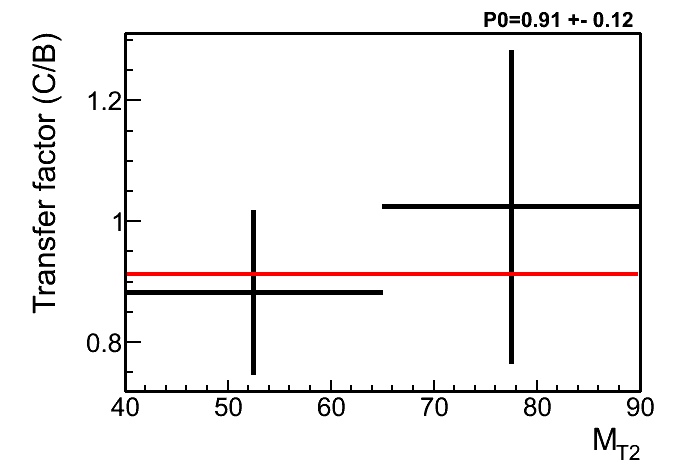
\includegraphics[width=0.49\textwidth]{QCDbginTauTau/Bin1-transferfactor.png}
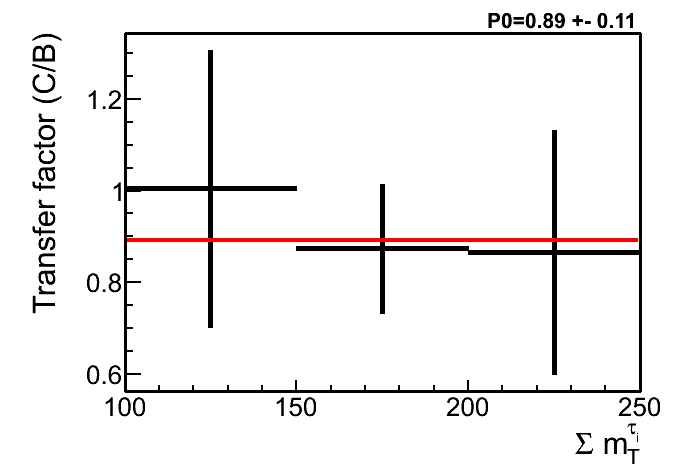
\includegraphics[width=0.49\textwidth]{QCDbginTauTau/Bin2-transferfactor.png} \\
\caption{The distribution of transfer factor as a function of \mttwo (left) and \SumMT (right). A $pol0$ function is used to fit the plots.}
\label{fig:1QCDbg}
\end{figure}

In order to increase the contributions from QCD events, the cut on the $\mindphifour>1$ is removed.
To consider the effect of this cut, a cut efficiency should be taken into account. The 
fraction of QCD events with all selection cuts with respect to the QCD events with all selection 
cuts but the $\mindphifour>1$ are shown in figure~\ref{fig:3QCDbg}.\\
\begin{figure}[!Hhtb]
\centering
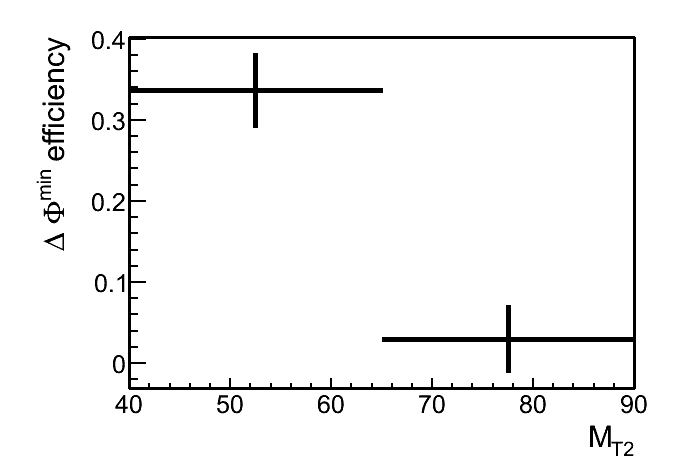
\includegraphics[width=0.49\textwidth]{QCDbginTauTau/Bin1-efficiency.png}
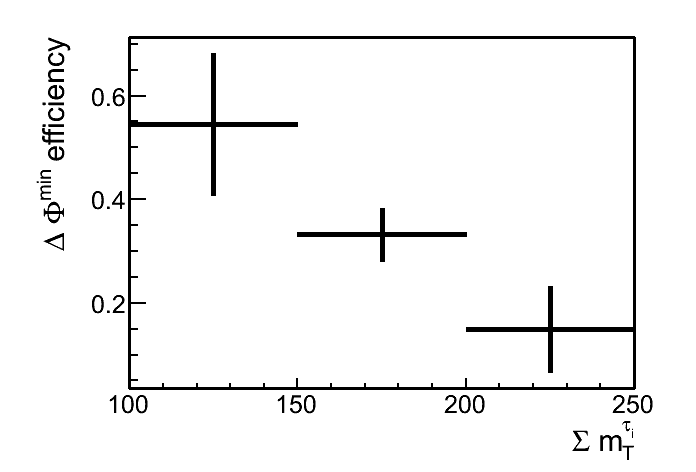
\includegraphics[width=0.49\textwidth]{QCDbginTauTau/Bin2-efficiency.png} \\
\caption{ The fraction of QCD events with all selection cuts with respect to the QCD events with all selection 
cuts but the $\mindphifour>1$ as a function of \mttwo (left) and \SumMT (right).}
\label{fig:3QCDbg}
\end{figure}

The value of the cut efficiency 
in the last bin is used to estimate the 
QCD background events in both signal regions. %While for the right plot, the distribution is fitted with a $pol1$ function to 
%take into account the fluctuations of the cut efficiencies in the first few bins. Then the cut efficiency extracted from 
%t%his plot is simply defined as the evaluation of the fit function at $\SumMT=250$. [{\bf FIXME} update this with comments from SUSY meeting] It should be noted that, performing such a 
%$pol1$% fit function on the left plot would yield to a negative value for the cut efficiency and then it was decided to  
%take the value in the last bin as a conservative estimate of the cut efficiency which is used in the final QCD background estimation results. 
The results of the ABCD method are summarized in table~\ref{4QCDbg}.\\

\begin{table}[!Hhtb]
\begin{center}
\caption{The ingredients needed for the ABCD method are summarized. The quoted 
uncertainties on data are statistical. For the nonQCD(MC) events, the systematical uncertainty  
 is also considered as 28\% of the central value. This systematical uncertainty is also propagated to the data subtraction. 
The final QCD background estimation results is shown in the last column.}
\scalebox{0.66}{
\begin{tabular}{|l|c|c|c|c|c|c|c|}
\hline\hline
 Region      & Sample   & RegionA    & RegionB     & RegionC     & T=C/B &$\mindphifour$efficiency& Estimation\\
\hline\hline
             & Susy     & 0.02$\pm$0.02  &0.07$\pm$0.04   &    10.68$\pm$0.57    &                       &         & \\
\binone      & Data      & 6.00$\pm$2.45 &  282.00$\pm$16.79   &330.00$\pm$18.17  &  0.91$\pm$0.12          &   0.03 $\pm$ 0.04 &0.13 $\pm$ 0.06(Stat)$\pm$ 0.19(Sys) $\pm$ 0.1(Fit Unc.) \\
             &NonQCD(MC)     & 1.19 $\pm$ 0.78  &  20.27$\pm$5.16  & 93.07$\pm$ 21.02  &             &                  &             \\
             &Data-NonQCD(MC)& 4.81$\pm$2.57    &261.73$\pm$17.71    &236.93$\pm$27.78   &             &                  &             \\
\hline
  & Susy          & 0.06$\pm$0.04 &  0.00$\pm$0.00 &  3.59$\pm$0.32 &            &                  &            \\
\bintwo     & Data          & 11.00 $\pm$ 3.32  &231.00$\pm$15.2&257.00$\pm$16.03&  0.89$\pm$0.11 & 0.15 $\pm$ 0.08     &1.15 $\pm$ 0.39(Stat) $\pm$ 0.7(Sys)$\pm$ 0.25 (Fit Unc.)          \\
             &NonQCD(MC)     & 2.38 $\pm$ 1.26  &14.5$\pm$ 4.07 & 65.1$\pm$13.53  &            &                &             \\
             &Data-NonQCD(MC)& 8.62 $\pm$3.55&  216.5$\pm$15.74    &  191.9$\pm$20.98     &     & &     \\ 
\hline\hline
\end{tabular}}
\label{4QCDbg}
\end{center}
\end{table}

Various sources of uncertainty are considered to determine the QCD background. 
In addition to the statistical uncertainties of data and MC, 28\% of 
nonQCD MC events is considered as systematic uncertainty.
Also an uncertainty due to the fit model has been assigned. Since we have used a pol0 fit 
to read the transfer factor and also take the value of the last bin from the $\mindphifour$ efficiency plot,
therefore an uncertainty originating from considering various fit models is evaluated. To do so, several 
fit models are examined and compared with our fit model. The uncertainty is defined to be as the 
difference between the central value of QCD events in signal region and a weighted mean value obtained from the formula below 
\begin{equation}
{\rm Weighted~mean~value} =\frac{\Sigma N_{QCD}/\varepsilon_{QCD}}{\Sigma 1/\varepsilon_{QCD}},
\end{equation}
\begin{equation}
{\rm Fit~uncertainty} ={\rm Weighted~mean~value}-{\rm the~central~value~of~QCD~events~in~SR},
\end{equation}

where $N_{QCD}$ and $\varepsilon_{QCD}$ are defined as the number of QCD events in signal region and 
the corresponding uncertainty, respectively. The sum is performed over various fit models.\\ 

In order to check how the ABCD method works, the distributions of the search variables are shown in 
figure~\ref{fig:5QCDbg}. The SM background distributions are taken from MC simulation, except for 
the QCD multi-jet contribution, which is estimated using the ABCD method. The \wjets background in the last bin of the \mttwo which is \binone of
analysis is estimated by the method described in Section \ref{sect:bkgW}.
\begin{figure}[iHhtb]
\centering
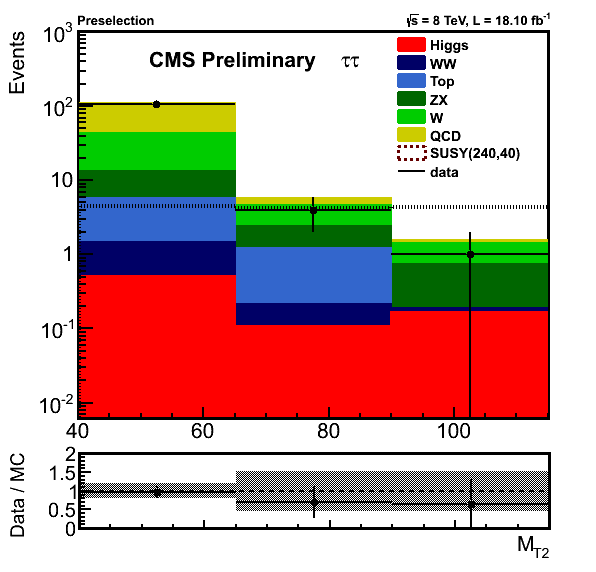
\includegraphics[angle=0,scale=0.375]{QCDbginTauTau/QCDWestimation_bin1.png}
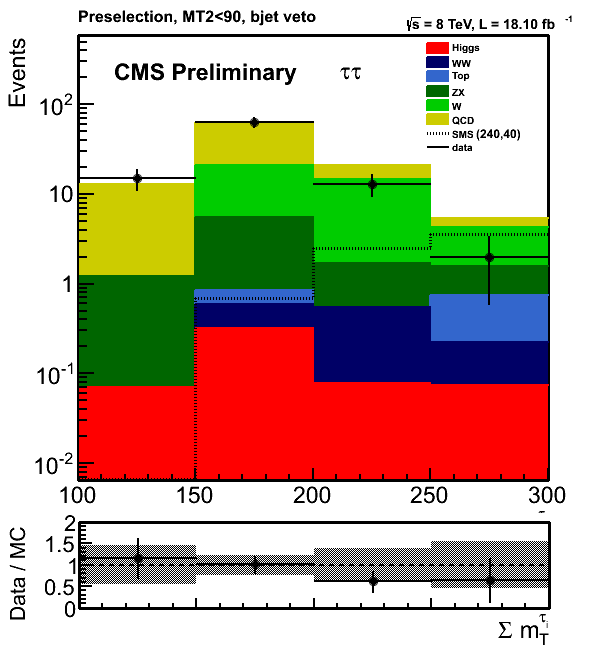
\includegraphics[angle=0,scale=0.375]{QCDbginTauTau/QCDWestimation_bin2.png}
\caption{The distributions of the \mttwo (left) and \SumMT (right) before the requirement on the given variable
is applied. The QCD multi-jet contribution is estimated from data using the ABCD method.}
\label{fig:5QCDbg}
\end{figure}
